\documentclass{classrep}
\usepackage[utf8]{inputenc}

\usepackage[pdftex]{color,graphicx}
\DeclareGraphicsExtensions{.pdf,.png,.jpg,.bmp}

\usepackage{float}
\usepackage{subfig}
\usepackage{color}
\usepackage{tabularx}

\usepackage{listings}

\usepackage{color}

\usepackage{url}

\usepackage{hyperref}

\usepackage[polish]{babel}

\usepackage{enumitem}
\usepackage{paralist}
\usepackage{indentfirst}

\hypersetup{colorlinks=false,pdfborder={0 0 0}}


\definecolor{javared}{rgb}{0.6,0,0} % for strings
\definecolor{javagreen}{rgb}{0.25,0.5,0.35} % comments
\definecolor{javapurple}{rgb}{0.5,0,0.35} % keywords
\definecolor{javadocblue}{rgb}{0.25,0.35,0.75} % javadoc

\lstset{language=Java,
basicstyle=\ttfamily,
keywordstyle=\color{javapurple}\bfseries,
stringstyle=\color{javared},
commentstyle=\color{javagreen},
morecomment=[s][\color{javadocblue}]{/**}{*/},
numbers=left,
numberstyle=\tiny\color{black},
stepnumber=2,
numbersep=10pt,
tabsize=4,
showspaces=false,
showstringspaces=false}


\studycycle{Informatyka, studia dzienne, mgr II st.}
\coursesemester{I}

\coursename{Przetwarzanie obrazu i dźwięku}
\courseyear{2011/2012}

\courseteacher{dr inż. Arkadiusz Tomczyk}
\coursegroup{środa, 8:15}

\author{
  \studentinfo{Paweł Musiał}{178726} \and
  \studentinfo{Łukasz Michalski}{178724}
}
\title{Zadanie 1:\\  \textbf {Szkielet aplikacji do przetwarzania \\i analizy obrazów, operacje podstawowe, usuwanie szumu, modyfikacje histogramu, filtracja liniowa i nieliniowa, splot}}
\svnurl{http://serce.ics.p.lodz.pl/svn/labs/poid/at_sr0800/lmpm}

\begin{document}
\maketitle

\addtocounter{footnote}{1}

\tableofcontents

\section{Cel}

Celem zadania było stworzenie szkieletu aplikacji służącej do wczytywania, zapisywania i  przetwarzania obrazów, która zostanie wykorzysta zarówno w tym, jak i w następnym zadaniu. Dodatkowo należało zaimplementować kilka filtrów i podstawowych operacji przetwarzania obrazów takich jak zmiana jasności, kontrastu czy odwrócenie kolorów obrazu. Pełny spis wymagań i przygotowanych filtrów został przedstawiony poniżej:

\begin{list}{•}{}
\item zaimplementować podstawowe operacje przetwarzania obrazów: zmianę jasności i kontrastu oraz wyznaczenie negatywu obrazu;
\item zaimplementować filtr ze średnią arytmetyczną i filtr medianowy z możliwością wyboru rozmiaru maski oraz zaproponować metody obiektywnej oceny ich działania i skuteczności w usuwaniu różnego rodzaju szumu;
\item wyznaczyć i wyświetlić histogram jasności pikseli obrazu, a w przypadku
obrazów kolorowych także histogram wartości poszczególnych kanałów;
\item w oparciu o wyznaczony histogram dokonać modyfikacji obrazu w taki sposób, aby osiągnąć zadaną charakterystykę histogramu obrazu wynikowego [(H3) Wyjściowa gęstość prawdopodobieństwa podana wzorem Raleigha];
\item zaimplementować możliwość filtracji liniowej opartej o splot w dwóch wersjach: na podstawie jednego z wariantów gotowych masek oraz z możliwością wyboru własnego rozmiaru maski i wartości poszczególnych jej elementów [(S6) Identyfikowanie linii];
\item opracować i zaimplementować algorytm filtracji nieliniowej obrazu w dziedzinie czasu zgodnie z regułą zawartą w przydzielonym wariancie zadania, a także zapewnić możliwość wyboru parametrów filtru tam, gdzie jest to konieczne [(O5) Operator Rosenfelda];
\end{list}

W sprawozdaniu zamieszczono wyniki działania poszczególnych algorytmów oraz porównanie ich pracy w różnych wariantach ustawień i~dla różnych problemów. Badania przeprowadzono zarówno na obrazach kolorowych (24-bitowych), jak i~w odcieniach szarości (8-bitowych), a~część badań również na obrazach czarno-białych (1-bitowych). 

\section{Wprowadzenie}
Obrazy przechowywane są w pamięci komputera w postaci bitowej, w której określa się ilość bitów przypadającą na każdy piksel obrazu. Kolorowe zdjęcia zapisywane są w formacie 24-bitowym co odpowiada 8-bitom na każdy~z trzech składowych kanałów formatu RGB. Fotografie w odcieniach szarości wykorzystują tylko jeden kanał dlatego wystarczy tutaj przechowywać 8-bitów na każdy zapisany piksel. Taki zapis umożliwia uzyskanie 256 różnych wartość danego piksela czyli 256 różnych odcieni szarości poczynając od białego na kolorze czarnym kończąc. W przypadku obrazów kolorowych liczba kombinacji jest dużo większa i wynosi 16,777,216, co nie oznacza, że wszystkie uzyskane w ten sposób kolory są między sobą rozróżnialne. W tej pracy wszystkie przygotowane algorytmy operują na poszczególnych wartościach każdego kanału obrazu.

\subsection{Zmiana jasności}
Zmiana jasności obrazu polega na zmniejszeniu bądź zwiększeniu składowych RGB o pewną wartość stałej b. Jeżeli jedna składowa uzyska wartość większą od dopuszczalnego zakresu to wynikiem jest wartość maksymalna z tego zakresu. Analogicznie, jeżeli składowa ma wartość mniejszą to wynikiem jest wartość minimalna. Powyższą operacją można zapisać za pomocą wzoru:
\begin{equation}
p(i)=\left\{
\begin{array}{l l l}
0 & \quad \mbox{i +b $<$ 0,} \\
i+b & \quad \mbox{0 $\leq$ i + b $\leq$  $i_{max}$,} \\
i_{max} & \quad \mbox{i + b $>$ $i_{max}$,} \\
\end{array}
\right.
\end{equation}
gdzie:
\begin{description}
\item $p(i)$ -- nowa wartość składowej RGB,
\item i -- wartość konkretnej składowej danego piksela,
\item b -- stała, o którą zmieniamy daną składową RGB,
\item $i_{max}$ -- maksymalna dopuszczalna wartość.
\end{description}

W przypadku obrazów czarno-białych (1-bitowych) zmiany jasności prowadzą do uzyskania całego białego bądź czarnego obrazu.
Przebieg zaprezentowanej tutaj funkcji zmiany jasności przedstawia (Rysunek \ref{fig:jasnosc}).

\begin{figure}[h!]
\centering
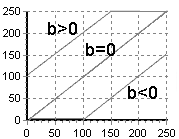
\includegraphics{obrazy/jasnosc.png} 
\caption[Zmiana jasności]{Przebiegi funkcji zmiany jasności z różną wartością stałej $b$.}
\label{fig:jasnosc}
\end{figure}

\subsection{Zmiana kontrastu}
Zmiana kontrastu polega na przekształceniu danego obrazu wykonując operację według wzoru:
\begin{equation}
\label{kontrastWzor}
p(i)=\left\{
\begin{array}{l l l}
0 & \quad \mbox{$a (i-\frac{i_{max}}{2}) + \frac{i_{max}}{2}$ $<$ 0,} \\
a (i-\frac{i_{max}}{2}) + \frac{i_{max}}{2} & \quad \mbox{0 $\leq$ $a (i-\frac{i_{max}}{2}) + \frac{i_{max}}{2}$ $\leq i_{max}$ ,} \\
i_{max} & \quad \mbox{$a (i-\frac{i_{max}}{2}) + \frac{i_{max}}{2}$ $ > i_{max}$,} \\
\end{array}
\right.
\end{equation}
gdzie:
\begin{description}
\item $p(i)$ -- nowa wartość składowej RGB,
\item i -- wartość konkretnej składowej danego piksela,
\item a -- stała, której wartość określa czy zwiększa się kontrast obrazu
\item $i_{max}$ -- maksymalna dopuszczalna wartość.
\end{description}

W przypadku jeżeli stała $a$ przyjmuje wartości większe od 1, następuje zwiększenie kontrastu obrazu. Natomiast, jeżeli wartości są mniejsze od 1 to kontrast jest zmniejszany. Przebieg zaprezentowanej tutaj funkcji zmiany kontrastu przedstawia (Rysunek \ref{fig:kontrast}).

\begin{figure}[h!]
\centering
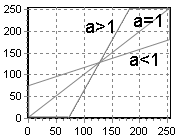
\includegraphics{obrazy/kontrast.png} 
\caption[Zmiana kontrastu]{Przebiegi funkcji zmiany kontrastu z różną wartością parametru $a$.}
\label{fig:kontrast}
\end{figure}

\subsection{Negatyw}
Wykonanie negatywu danego obrazu polega na przekształceniu wszystkich pikseli za pomocą wzoru:
\begin{equation}
 p(i) = i_{max} - i
\end{equation}
gdzie:
\begin{description}
\item $p(i)$ -- nowa wartość składowej RGB,
\item $i_{max}$ -- maksymalna dopuszczalna wartość,
\item i -- wartość konkretnej składowej danego piksela.
\end{description}

Tą operację należy wykonać na każdym z kanałów z osobna w celu uzyskania pełnego negatywu w przypadku np. zdjęć kolorowych.

\subsection{Filtr ze średnią arytmetyczną}

Filtracja za pomocą tego algorytmu polega na wybraniu wielkości okna maski (w środku okna znajduje się piksel aktualnie przetwarzany). Kolejnym krokiem jest uśrednienie wartości poszczególnych pikseli w danym oknie. Dla obrazu kolorowego algorytm wykonujemy dla każdego kanału osobna. Np. dla maski rozmiaru 3x3 uśredniane są wartości 9 pikseli. Efekt działania tego filtru przedstawia (Rysunek \ref{fig:meanFilter}).
\begin{figure}[h!]
\centering
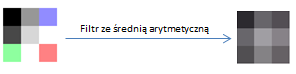
\includegraphics[width=7.83cm]{obrazy/meanFilter.png} 
\caption[Filtr ze średnią arytmetyczną]{Przykład działania filtru ze średnią arytmetyczną z maską rozmiaru 3x3.}
\label{fig:meanFilter}
\end{figure}

\subsection{Filtr medianowy}
Algorytm podobny do filtracji ze średnią arytmetyczną jednak zamiast uśredniana wartości poszczególnych pikseli w masce wybierana jest ich mediana czyli wartość środkowa z uszeregowanego rosnąco ciągu wszystkich wartości. Dla obrazu kolorowego algorytm również wykonywany jest dla każdego kanału osobno. Efekt działania tego filtru przedstawia (Rysunek \ref{fig:medianFilter}).
\begin{figure}[h!]
\centering
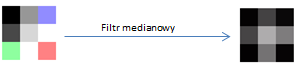
\includegraphics[width=7.89cm]{obrazy/medianFilter.png} 
\caption[Filtr medianowy]{Przykład działania filtru medianowego z maską rozmiaru 3x3.}
\label{fig:medianFilter}
\end{figure}

\subsection{Generowanie i modyfikacja histogramu}
Aby wygenerować histogram należy zebrać informacje o tym ile pikseli w danym kolorze znajduje się na obrazie (dla obrazu kolorowego każdy kanał badamy osobno). Po zsumowaniu wszystkich pikseli generowany jest wykres słupkowy gdzie na osi X znajdują się kolejne wartości jakie może przyjąć kolor a na osi Y ilość pikseli w danym kolorze na obrazie.

Dla obrazu w odcieniach szarości i czarno-białego generowany jest jeden histogram natomiast dla kolorowego cztery. Trzy z nich to reprezentują kolejne kanały obrazu (czerwony, zielony i niebieski) a jeden dodatkowy to histogram wartości luminacji dla danego piksela liczona według wzoru:
\begin{equation}
 y = 0,299r + 0,587g + 0,114b, \label{luminacja}
 \end{equation}
gdzie:
\begin{description}
\item y -- wartość luminacji dla danego piksela,
\item r -- wartość kanału czerwonego dla danego piksela,
\item g -- wartość kanału zielonego dla danego piksela,
\item b -- wartość kanału niebieskiego dla danego piksela.
\end{description}

\subsection{Filtracja liniowa -- identyfikowanie linii}
Filtracja liniowa poleca na przekształceniu obrazu wejściowego poprzez nakładanie maski o określonym rozmiarze i wagach poszczególnych pikseli w masce.
\begin{matrix}

\begin{tabular}{|c|c|c|}
\hline -1 & 2 & -1 \\ 
\hline -1 & 2 & -1 \\ 
\hline -1 & 2 & -1 \\ 
\hline 
\end{tabular} 

\begin{tabular}{|c|c|c|}
\hline -1 & -1 & -1 \\ 
\hline 2 & 2 & 2 \\ 
\hline -1 & -1 & -1 \\ 
\hline 
\end{tabular} 

\begin{tabular}{|c|c|c|}
\hline -1 & -1 & 2 \\ 
\hline -1 & 2 & -1 \\ 
\hline 2 & -1 & -1 \\ 
\hline 
\end{tabular} 

\begin{tabular}{|c|c|c|}
\hline 2 & -1 & -1 \\ 
\hline -1 & 2 & -1 \\ 
\hline -1 & -1 & 2 \\ 
\hline 
\end{tabular} 


W naszym przypadku wagi są ustanowione tak, aby w obrazie w miejscach gdzie występują linie odpowiadające orientacji wag dodatnich nastąpiło wzmocnienie, a gdzie ujemne osłabienie. W ten sposób na obrazie wynikowym otrzymujemy wykryte linie zaznaczone jaśniejszymi odcieniami, a tam gdzie ich nie wykryto obszary zacienione.


\subsection{Filtracja nieliniowa -- operator Rosenfelda}
Filtracja nieliniowa realizująca operator Rosenfelda o wzorze :
\begin{equation}
g(x,y)=\frac{1}{R}\left( \sum \limits _{i=1} ^{R} f \left( x+i-1,y \right) - \sum \limits _{i=1} ^{R} f \left(x-i,y \right) \right)
\end{equation}
Dla piksela wejściowego, wyjściem będzie uśredniona wartość różnicy elementów powyżej i poniżej wejściowego rozpatrywanego elementu. W wyniku daje nam do metodę identyfikacji krzywych na obrazie. jeśli punkt leży na pograniczu dwóch dwóch nasyceń różnica będzie duża, dzięki czemu uzyskamy w danym punkcie jasny obszar, a przeciwnym wypadku, będzie to obszar zacieniony.


\subsection{Miary podobieństwa}
Aby dokładnie określić jak bardzo dwa obrazy się od siebie różnią zastosowaliśmy szereg miar podobieństwa, które wyliczamy w trakcie pracy programu. Mają one nam pozwolić na obiektywne stwierdzenie jakości poprawy przetworzonego za pomocą filtrów obrazu i porównanie go z obrazem początkowym.

\subsubsection*{Błąd średniokwadratowy (MSE)}
Błąd średniokwadratowy (MSE) określony jest wzorem:
\begin{equation}
 MSE = \frac{1}{N M}\sum\limits_{i=1}^N \sum\limits_{j=1}^M ([f(i,j)-f'(i,j)]^2) 
\end{equation}
gdzie:
\begin{description}
 \item $N,M$ -- wymiary obrazka
 \item $f(x,y)$ -- wartość piksela obrazu wzorcowego
 \item $f'(x,y)$ -- wartość piksela obrazu badanego
\end{description}

Im wartość tego błędu jest większa tym porównywane obrazy bardziej się od siebie różnią.

\subsubsection*{Szczytowy stosunek sygnału do szumu (PSNR)}
Kolejną wykorzystywaną przez nas miarą podobieństwa jest szczytowy stosunek sygnału do szumu (PSNR) wyrażony w dB:
\begin{equation}
 PSNR = 10 \log_{10}\frac{k^2}{MSE}
\end{equation}
gdzie:
\begin{description}
 \item $k$ -- liczba kolorów obrazu minus 1(w naszym przypadku 255)
\end{description}

W przypadku tej miary podobieństwa im większa otrzymana wartość określająca stosunek sygnału do szumy tym bardziej dwa porównywane obrazy są do siebie podobne. Wartość ta powinna zatem rosnąć wraz s poprawą jakość bądź też niwelacją szumu w obrazie pierwotnym.

\subsubsection*{Średni błąd bezwzględny (MAE)}
Średni błąd bezwzględny (MAE) określony jest wzorem:
\begin{equation}
 MAE = \frac{1}{N M}\sum\limits_{i=1}^N \sum\limits_{j=1}^M (|[f(i,j)-f'(i,j)]|) 
\end{equation}
gdzie:
\begin{description}
 \item $N,M$ -- wymiary obrazka
 \item $f(x,y)$ -- wartość piksela obrazu wzorcowego
 \item $f'(x,y)$ -- wartość piksela obrazu badanego
\end{description}

W porównaniu do wartości błędu średniokwadratowego, ta miara dopasowania jest mniej czuła na wartości odstające, to znaczy wyjątkowo duże wartości błędu będą wpływać na wartość MAE w mniejszym stopniu niż na wartość MSE.

\section{Opis implementacji}


\section{Materiały i metody}
W tym miejscu należy opisać, jak przeprowadzone zostały wszystkie badania,
których wyniki i dyskusja zamieszczane są w dalszych sekcjach. Opis ten
powinien być na tyle dokładny, aby osoba czytająca go potrafiła wszystkie
przeprowadzone badania samodzielnie powtórzyć w celu zweryfikowania ich
poprawności (a zatem m.in. należy zamieścić tu opis architektury sieci,
wartości współczynników użytych w kolejnych eksperymentach, sposób
inicjalizacji wag, metodę uczenia itp. oraz informacje o danych, na których
prowadzone były badania). Przy opisie należy odwoływać się i stosować do
opisanych w sekcji drugiej wzorów i oznaczeń, a także w jasny sposób opisać
cel konkretnego testu. Najlepiej byłoby wyraźnie wyszczególnić (ponumerować)
poszczególne eksperymenty tak, aby łatwo było się do nich odwoływać dalej.

\section{Wyniki}

\subsection{Wyniki odszumiania}

%% ODSZUMIANIE FILTREM UŚREDNIAJĄCYM ZDJĘCIA CZARNO-BIAŁE

\subsubsection{Filtr uśredniający}

 \begin{figure}[H]
  \centering
  \subfloat[szum pulsacyjny, uśrednienie wartości 5x5px]{
	  \label{avg:bwimpulse}
	  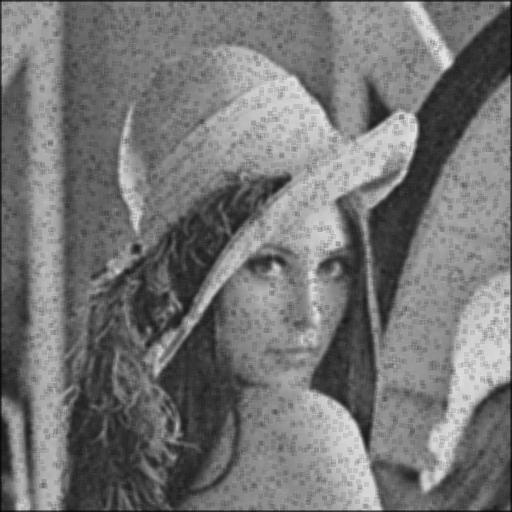
\includegraphics[width=0.3\textwidth]{testy/szum/mean/bw/lena_impulse2_p=5}
  }
  \subfloat[szum jednorodny uśrednienie wartości 3x3px]{
  		\label{avg:bwuniform}
  		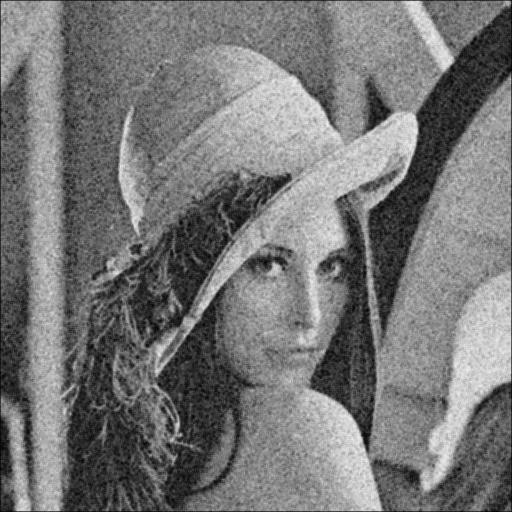
\includegraphics[width=0.3\textwidth]{testy/szum/mean/bw/lena_uniform3_p=3}
  	}
  \subfloat[szum normalny uśrednienie wartości 3x3px]{
  		\label{avg:bwnormal}
  		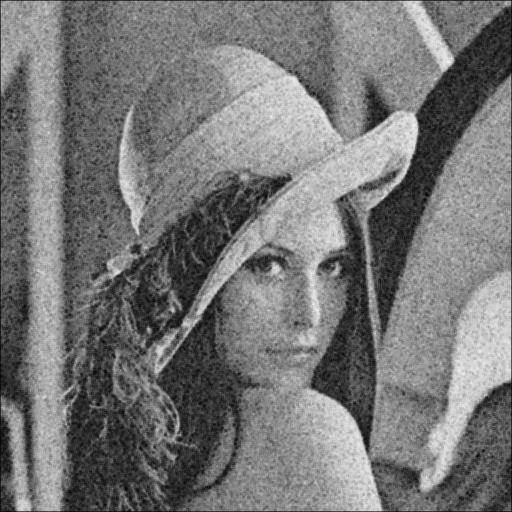
\includegraphics[width=0.3\textwidth]{testy/szum/mean/bw/lena_normal3_p=3}
  }
  \caption{Odszumianie zdjęć czarno-białych filtrem uśredniajacym.}
  \label{avg:bw}
\end{figure}

\begin{table}[H]
	\begin{center}
		\begin{tabular}{|l|l|l|l|l|l|l|}
			\hline
			obraz & MSE przed & PSNR przed & MAE przed & MSE po & PSNR po & MAE po \\
			\hline
			a & 923.99 & 18.47 & 16.91 & 149.42 & 26.38 & 22.79 \\
			b & 1044.60 & 17.94 & 47.43 & 181.45 & 25.54 & 28.14 \\
			c & 1007.17 & 18.09 & 37.56 & 172.87 & 25.75 & 27.34 \\
			\hline
		\end{tabular}
		\caption{Wartość współczynników zaszumienia dla rysunku \ref{avg:bw}.}
			\label{avgtab:bw}
	\end{center}

\end{table}


%% ODSZUMIANIE FILTREM UŚREDNIAJĄCYM ZDJĘCIA KOLOROWE

 \begin{figure}[H]
  \centering
  \subfloat[szum pulsacyjny, uśrednienie wartości 5x5px]{
	  \label{avg:colimpulse}
	  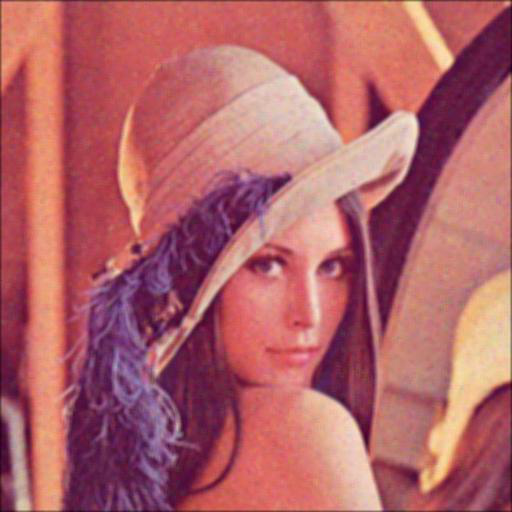
\includegraphics[width=0.3\textwidth]{testy/szum/mean/color/lena_impulse2_p=5}
  }
  \subfloat[szum jednorodny uśrednienie wartości 3x3px]{
  		\label{avg:coluniform}
  		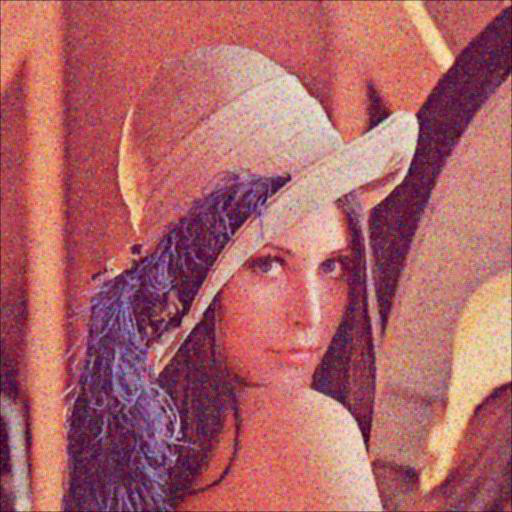
\includegraphics[width=0.3\textwidth]{testy/szum/mean/color/lena_uniform3_p=3}
  	}
  \subfloat[szum normalny uśrednienie wartości 3x3px]{
  		\label{avg:colnormal}
  		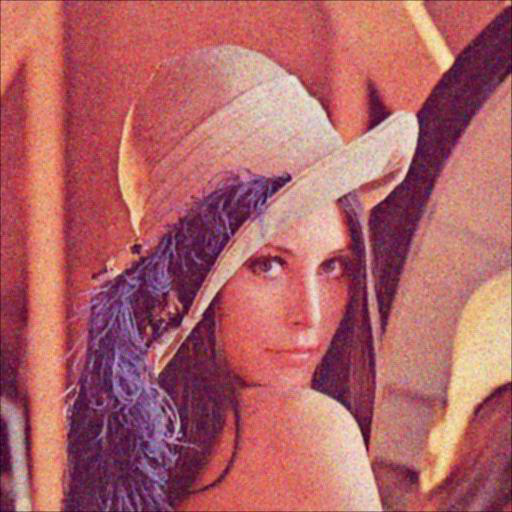
\includegraphics[width=0.3\textwidth]{testy/szum/mean/color/lena_normal3_p=3}
  }
  \caption{Odszumianie zdjęć kolorowych filtrem uśredniajacym.}
  \label{avg:col}
\end{figure}

\begin{table}[H]
	\begin{center}
		\begin{tabular}{|l|l|l|l|l|l|l|}
			\hline
			obraz & MSE przed & PSNR przed & MAE przed & MSE po & PSNR po & MAE po \\
			\hline
			a & 9577.64 & 20.51 & 13.99 & 125.89 & 27.13 & 21.12 \\
			b & 1738.53 & 15.72 & 58.27 & 253.08 & 24.09 & 36.35 \\
			c & 1090.84 & 17.75 & 51.92 & 169.58 & 25.83 & 29.79\\
			\hline
		\end{tabular}
		\caption{Wartość współczynników zaszumienia dla rysunku \ref{avg:col}.}
			\label{avgtab:col}
	\end{center}

\end{table}




%% ODSZUMIANIE FILTREM MEDIANOWYM ZDJĘCIA CZARNO-BIAŁE

\subsubsection{Filtr medianowy}

 \begin{figure}[H]
  \centering
  \subfloat[szum pulsacyjny, mediana wartości 3x3px]{
	  \label{men:bwimpulse}
	  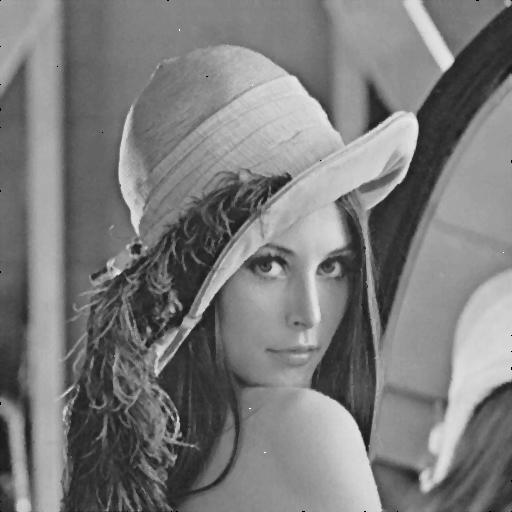
\includegraphics[width=0.3\textwidth]{testy/szum/median/bw/lena_impulse3_p=3}
  }
  \subfloat[szum jednorodny mediana wartości 3x3px]{
  		\label{men:bwuniform}
  		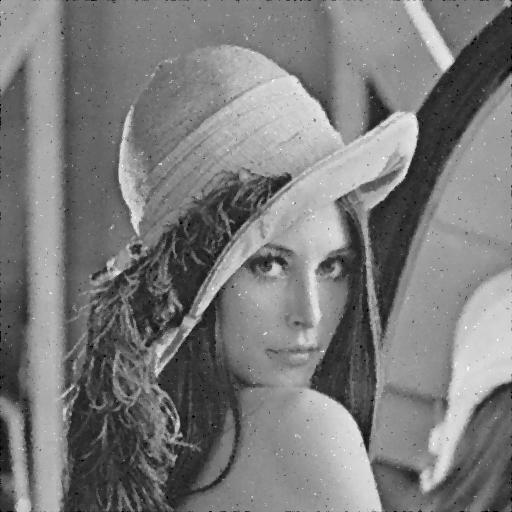
\includegraphics[width=0.3\textwidth]{testy/szum/median/bw/lena_uniform3_p=3}
  	}
  \subfloat[szum normalny mediana wartości 3x3px]{
  		\label{men:bwnormal}
  		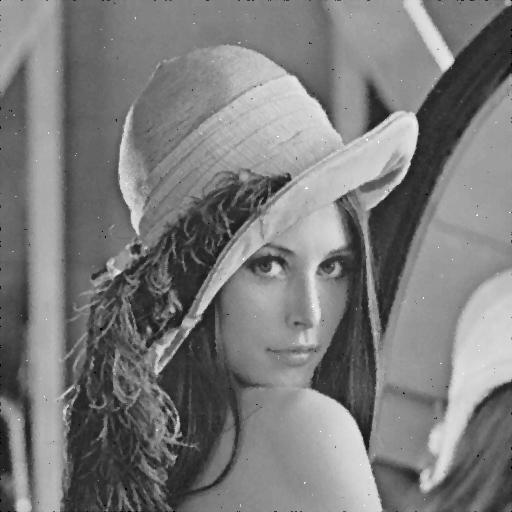
\includegraphics[width=0.3\textwidth]{testy/szum/median/bw/lena_normal3_p=3}
  }
  \caption{Odszumianie zdjęć czarno-białych filtrem medianowym.}
  \label{men:bw}
\end{figure}

\begin{table}[H]
	\begin{center}
		\begin{tabular}{|l|l|l|l|l|l|l|}
			\hline
			obraz & MSE przed & PSNR przed & MAE przed & MSE po & PSNR po & MAE po \\
			\hline
			a & 1762.70 & 15.66 & 33.14 & 21.43 & 34.82 & 5.19 \\
			b & 1044.60 & 17.94 & 47.43 & 48.50 & 31.27 & 9.15 \\
			c & 1007.17 & 18.09 & 37.56 & 29.57 & 33.42 & 6.54 \\
			\hline
		\end{tabular}
		\caption{Wartość współczynników zaszumienia dla rysunku \ref{men:bw}.}
			\label{mentabbw}
	\end{center}

\end{table}


%% ODSZUMIANIE FILTREM MEDIANOWYM ZDJĘCIA KOLOROWE

 \begin{figure}[H]
  \centering
  \def\tabularxcolumn#1{m{#1}}
\begin{tabularx}{\linewidth}{@{}cXX@{}}
%
\begin{tabular}{cc}

  \subfloat[szum pulsacyjny, mediana wartości 3x3px]{
	  \label{men:colimpulse}
	  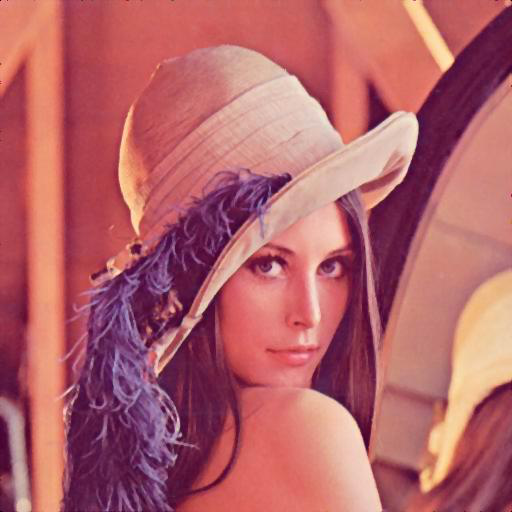
\includegraphics[width=0.48\textwidth]{testy/szum/median/color/lena_impulse3_p=3}
  } &
  \subfloat[szum jednorodny mediana wartości 3x3px]{
  		\label{men:coluniform}
  		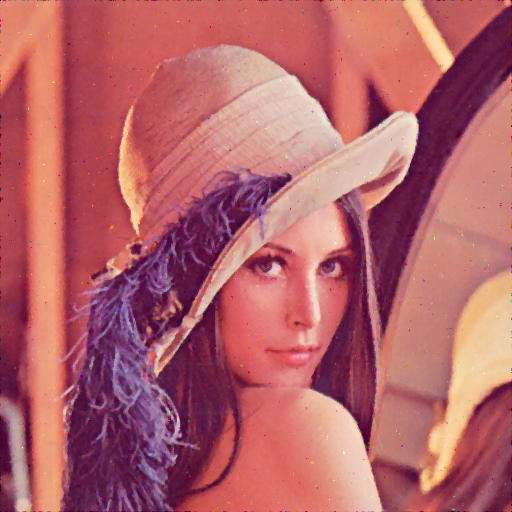
\includegraphics[width=0.48\textwidth]{testy/szum/median/color/lena_uniform3_p=3}
  	}\\
  \subfloat[szum jednorodny mediana wartości 5x5px]{
  		\label{men:coluniform2}
  		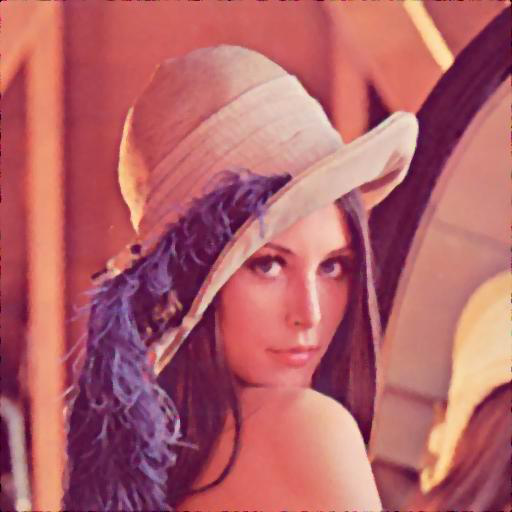
\includegraphics[width=0.48\textwidth]{testy/szum/median/color/lena_uniform3_p=5}
  	}&
  \subfloat[szum normalny uśrednienie wartości 3x3px]{
  		\label{men:colnormal}
  		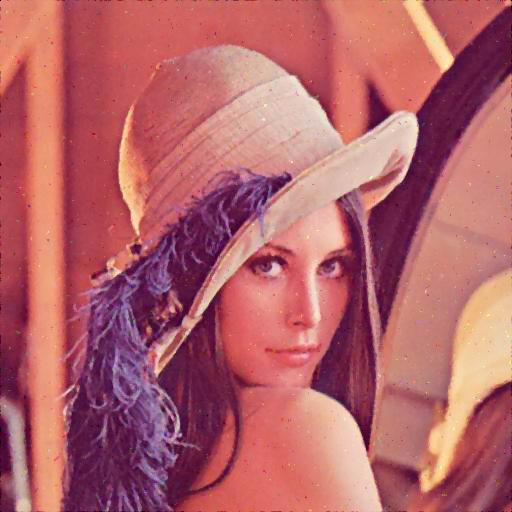
\includegraphics[width=0.48\textwidth]{testy/szum/median/color/lena_normal3_p=3}
  }\\
  \end{tabular}

  \end{tabularx}

  \caption{Odszumianie zdjęć kolorowych filtrem medianowym.}
  \label{men:col}
\end{figure}

\begin{table}[H]
	\begin{center}
		\begin{tabular}{|l|l|l|l|l|l|l|}
			\hline
			obraz & MSE przed & PSNR przed & MAE przed & MSE po & PSNR po & MAE po \\
			\hline
			a & 866.83 & 18.75 & 20.99 & 21.95 & 34.71 & 6.29 \\
			b & 1738.53 & 15.72 & 58.27 & 56.22 & 30.63 & 9.98 \\
			c & 1738.53 & 15.72 & 58.27 & 72.11 & 29.55 & 12.71\\
			d & 1090.84 & 17.75 & 51.92 & 67.27 & 29.85 & 10.78\\
			\hline
		\end{tabular}
		\caption{Wartość współczynników zaszumienia dla rysunku \ref{men:col}.}
			\label{mentabcol}
	\end{center}

\end{table}

\subsection{Filtracja liniowa}

 \begin{figure}[H]
  \centering
  \def\tabularxcolumn#1{m{#1}}
\begin{tabularx}{\linewidth}{@{}cXX@{}}
%
\begin{tabular}{cc}

  \subfloat[wykrywanie linii poziomych]{
	  \label{line:linearA1}
	  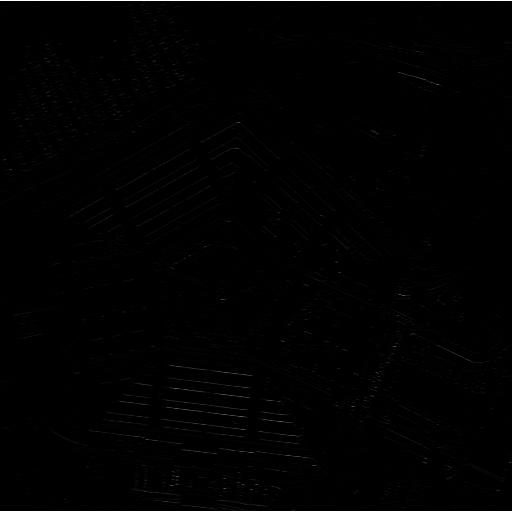
\includegraphics[width=0.37\textwidth]{testy/filtr_liniowy/pentagon1}
  } &
  \subfloat[wykrywanie linii pionowych]{
  		\label{line:linearA2}
  		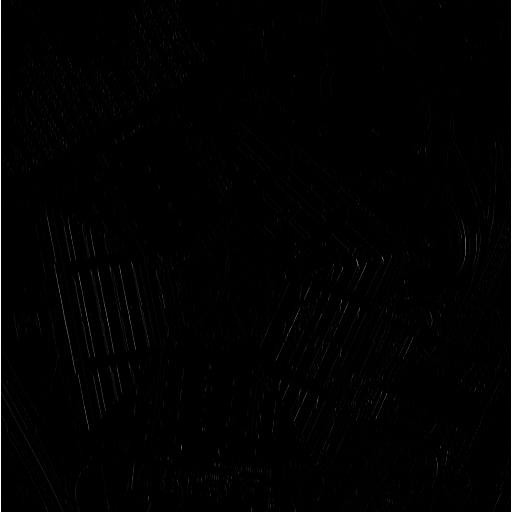
\includegraphics[width=0.37\textwidth]{testy/filtr_liniowy/pentagon2}
  	}\\
  \subfloat[wykrywanie linii skośnych]{
  		\label{line:linearA3}
  		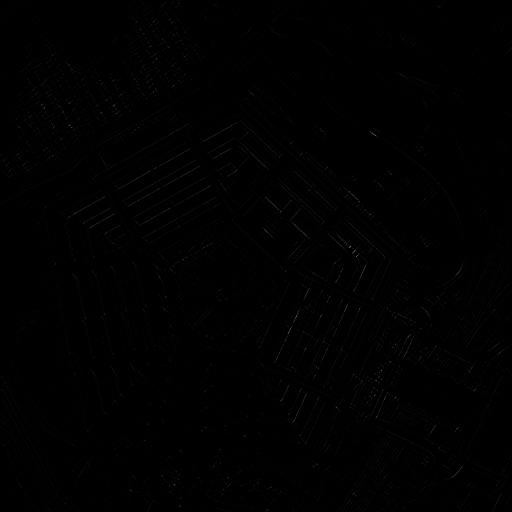
\includegraphics[width=0.37\textwidth]{testy/filtr_liniowy/pentagon3}
  	}&
  \subfloat[wykrywanie linii skośnych]{
  		\label{line:linearA4}
  		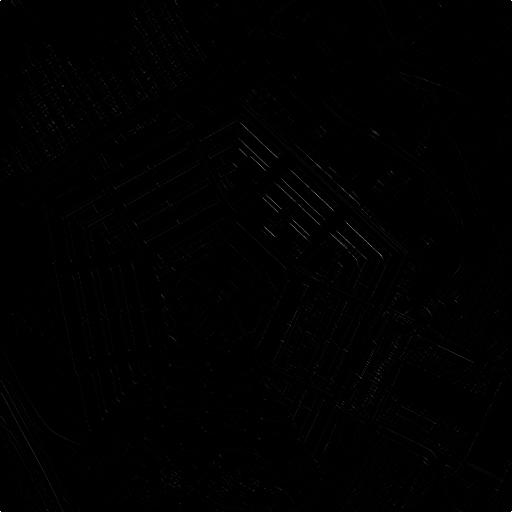
\includegraphics[width=0.37\textwidth]{testy/filtr_liniowy/pentagon4}
  }\\
  \end{tabular}

  \end{tabularx}

  \caption{Filtr liniowy, wykrywanie linii, obraz ,,pentagon''.}
  \label{line:linearA}
\end{figure}


 \begin{figure}[H]
  \centering
  \def\tabularxcolumn#1{m{#1}}
\begin{tabularx}{\linewidth}{@{}cXX@{}}
%
\begin{tabular}{cc}


  \subfloat[wykrywanie linii poziomych]{
	  \label{line:linearB1}
	  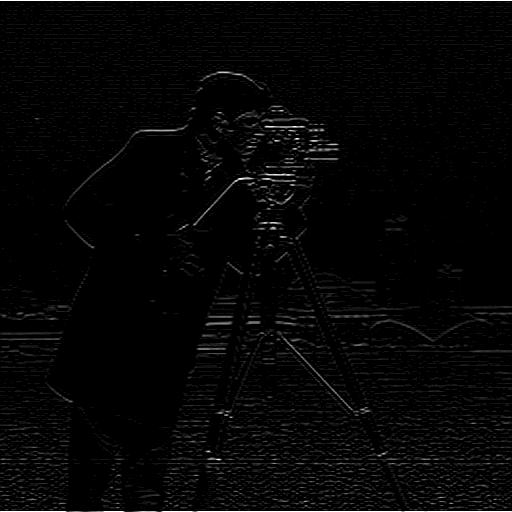
\includegraphics[width=0.37\textwidth]{testy/filtr_liniowy/camera1}
  } &
  \subfloat[wykrywanie linii pionowych]{
  		\label{line:linearB2}
  		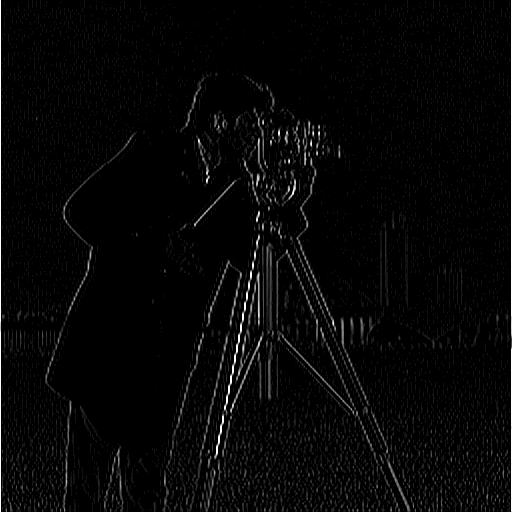
\includegraphics[width=0.37\textwidth]{testy/filtr_liniowy/camera2}
  	}\\
  \subfloat[wykrywanie linii skośnych]{
  		\label{line:linearB3}
  		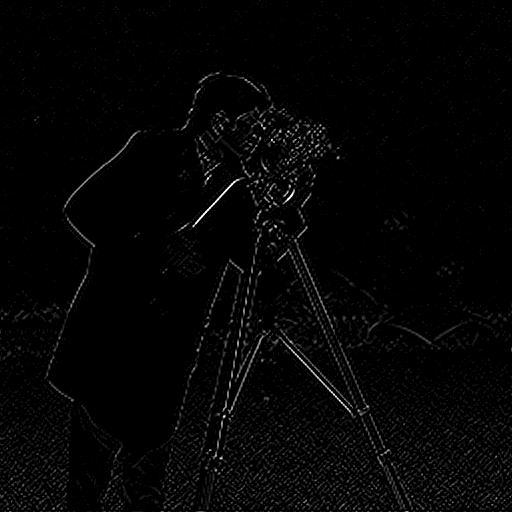
\includegraphics[width=0.37\textwidth]{testy/filtr_liniowy/camera3}
  	}&
  \subfloat[wykrywanie linii skośnych]{
  		\label{line:linearB4}
  		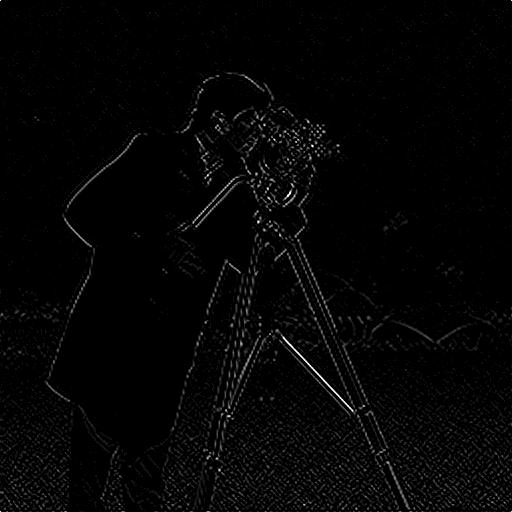
\includegraphics[width=0.37\textwidth]{testy/filtr_liniowy/camera4}
  }\\
  \end{tabular}

  \end{tabularx}

  \caption{Filtr liniowy, obraz ,,camera''.}
  \label{line:linearB}
\end{figure}

\subsection{Filtracja nieliniowa}
 \begin{figure}[H]
  \centering
  \def\tabularxcolumn#1{m{#1}}
\begin{tabularx}{\linewidth}{@{}cXX@{}}
%
\begin{tabular}{cc}
  \subfloat[wykrywanie linii poziomych]{
	  \label{line:nlinearA1}
	  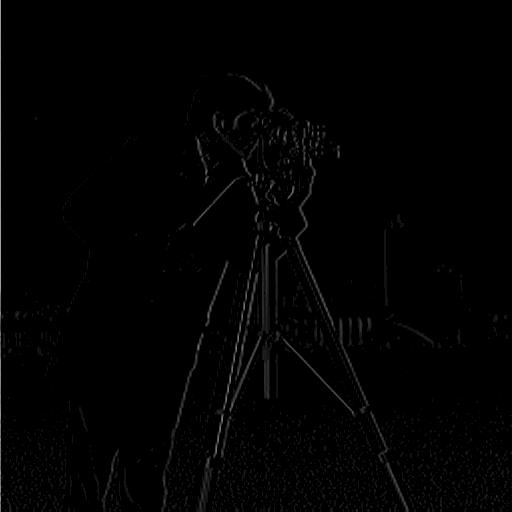
\includegraphics[width=0.37\textwidth]{testy/filtr_nieliniowy/camera}
  } & 
  \subfloat[wykrywanie linii pionowych]{
  		\label{line:nlinearA2}
  		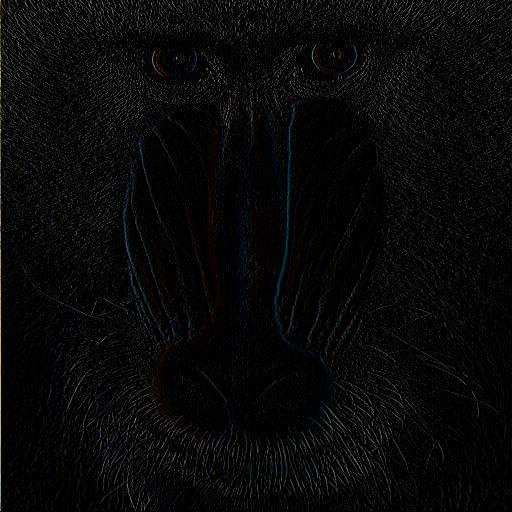
\includegraphics[width=0.37\textwidth]{testy/filtr_nieliniowy/mandrilc}
  	}\\
  	  \subfloat[wykrywanie linii pionowych]{
  		\label{line:nlinearA3}
  		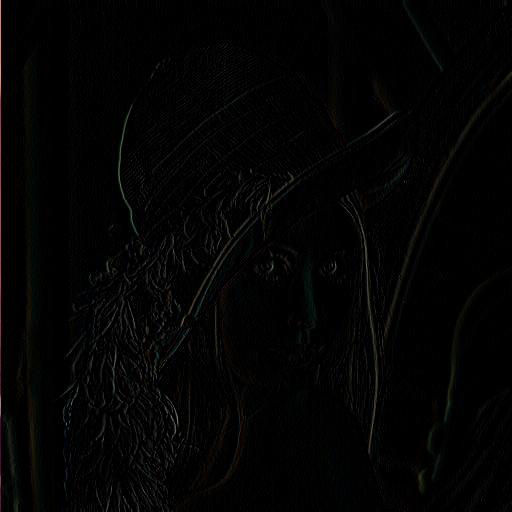
\includegraphics[width=0.37\textwidth]{testy/filtr_nieliniowy/lenac}
  	}\\
  	  \end{tabular}

  \end{tabularx}

  \caption{Filtr nieliniowy, obraz ,,camera'' , ,,mandrilc'' oraz ,,lenac''.}
  \label{line:nlinear}
\end{figure}


\subsection{Modyfikacja histogramowa}
 \begin{figure}[H]
  \centering
  \def\tabularxcolumn#1{m{#1}}
\begin{tabularx}{\linewidth}{@{}cXX@{}}
%
\begin{tabular}{cc}


  \subfloat[obraz oryginalny]{
	  \label{raleight:lena_in}
	  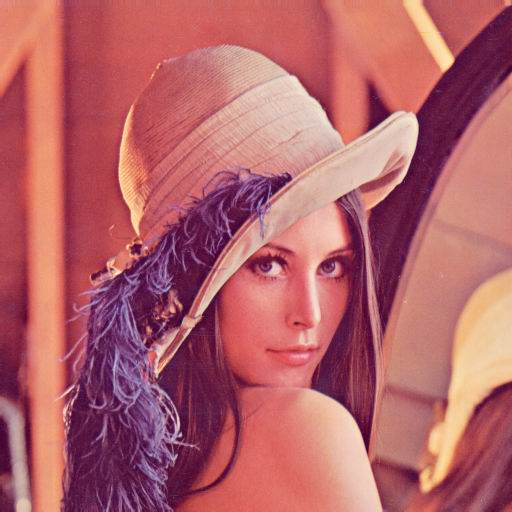
\includegraphics[width=0.37\textwidth]{testy/raleight/lenac}
  } &
  \subfloat[histogram obrazu oryginalnego]{
  		\label{raleight:lena_inhist}
  		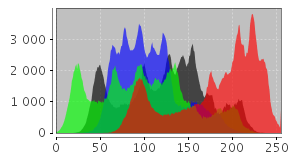
\includegraphics[width=0.37\textwidth]{testy/raleight/lenac_in_hist}
  	}\\
  \subfloat[obraz po przekształceniu]{
  		\label{raleight:lena_out}
  		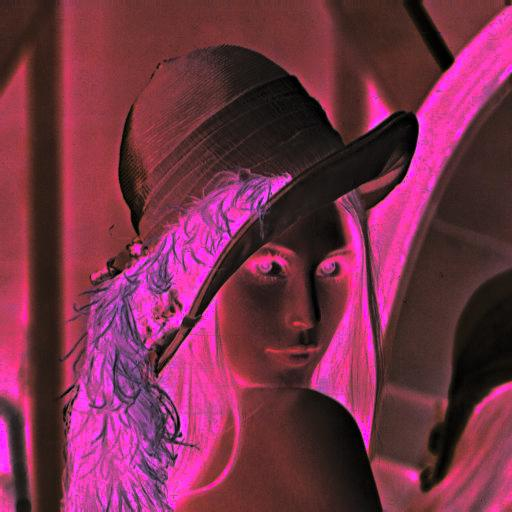
\includegraphics[width=0.37\textwidth]{testy/raleight/lenac_out}
  	}&
  \subfloat[histogram obrazu przekształconego]{
  		\label{raleight:lena_outhist}
  		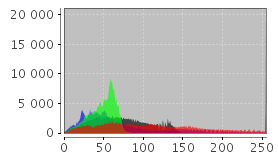
\includegraphics[width=0.37\textwidth]{testy/raleight/lenac_out_hist}
  }\\
  \end{tabular}

  \end{tabularx}

  \caption{Przekształcenie histogramowe obrazu ,,lenac'' parametr gmin=0, alpha oszacowany automatycznie.}
  \label{raleight:lena}
\end{figure}

 \begin{figure}[H]
  \centering
  \def\tabularxcolumn#1{m{#1}}
\begin{tabularx}{\linewidth}{@{}cXX@{}}
%
\begin{tabular}{cc}


  \subfloat[obraz oryginalny]{
	  \label{raleight:mandrilc_in}
	  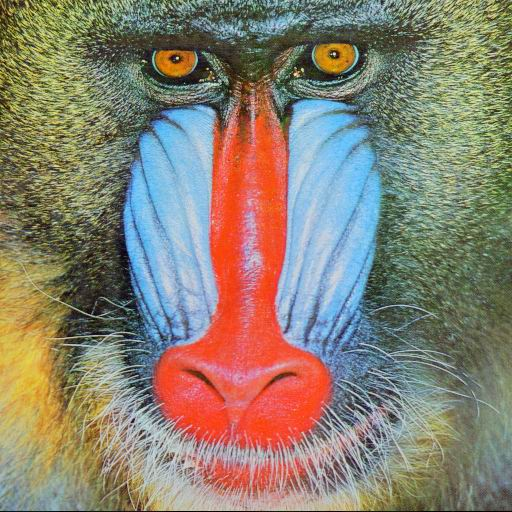
\includegraphics[width=0.37\textwidth]{testy/raleight/mandrilc}
  } &
  \subfloat[histogram obrazu oryginalnego]{
  		\label{raleight:mandrilc_inhist}
  		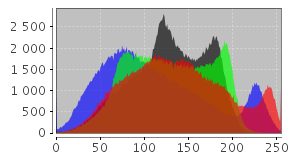
\includegraphics[width=0.37\textwidth]{testy/raleight/mandrilc_in_hist}
  	}\\
  \subfloat[obraz po przekształceniu]{
  		\label{raleight:mandrilc_out}
  		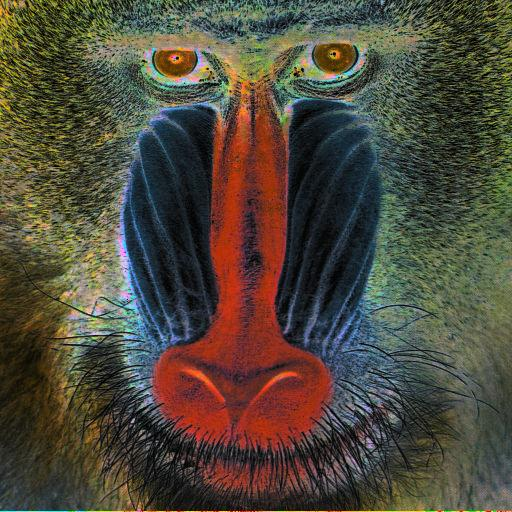
\includegraphics[width=0.37\textwidth]{testy/raleight/mandrilc_out}
  	}&
  \subfloat[histogram obrazu przekształconego]{
  		\label{raleight:mandrilc_outhist}
  		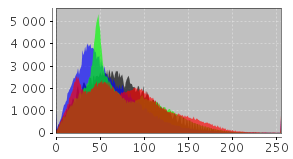
\includegraphics[width=0.37\textwidth]{testy/raleight/mandrilc_out_hist}
  }\\
  \end{tabular}

  \end{tabularx}

  \caption{Przekształcenie histogramowe obrazu ,,mandrilc'' parametr gmin=0, alpha oszacowany automatycznie.}
  \label{raleight:mandrilc}
\end{figure}


\section{Dyskusja}

\subsection{Odszumianie}

W większości przypadków, zebrane tutaj dane wynikowe dotyczą wariantów najbardziej zaszumionych z każdego rodzaju szumi. Dobrano takie przykładu aby uwypuklić różnice pomiędzy metodami.

\subsubsection{Filtr uśredniający}

Filtr uśredniający niestety nie radzi sobie zbyt dobrze z żadnym rodzajem szumu. Coraz to lepsze efekty daje dopiero, gdy bierzemy większe otoczenie do uśrednienia, lecz skutkuje rozmyciem obrazu, zanikają wyraźne krawędzie, co może być bardzo dużym minusem jeśli zdjęcie ma służyć dalszej obróbce. Przykładem takich zabiegów mogą być zdjęcia \ref{avg:bwimpulse} oraz \ref{avg:colimpulse}. Obrazy te wydają się być umiarkowanie odszumione, lecz straciliśmy na ich dokładności. W standardowym przypadku gdy bierzemy pod uwagę matryce 3x3px nie ma zauważalnej różnicy w wyrazistości  Wyniki badań  przyjętymi wskaźnikami zaszumienia zestawione w tabelach \ref{avgtab:bw} , \ref{avgtab:col} pokazują, że nasza subiektywna ocena może się czasem mylić, obrazy tak naprawdę są w pewnym stopniu odszumione, niestety dla naszego oka efekt jest niezadowalający.

\subsubsection{Filtr medianowy}

W porównaniu do wyżej wymienionej metody odszumiania obrazu ,,filtru uśredniającego'', metoda ta daje zaskakująco dobre efekty, w niektórych przypadkach, nie da się zauważyć różnic pomiędzy obrazem oryginalnym a obrazem odszumionym. Jak można zauważyć 
na rysunku \ref{men:bw} na pierwszy rzut oka trudno zauważyć jakąkolwiek różnice pomiędzy obrazami. Podobnie jest na rysunku \ref{men:col}, jednaj tutaj można już zauważyć pewne artefakty (widoczne na rys \ref{men:colnormal} i rys. \ref{men:coluniform}) zaistniałe z wyniku zastosowania tejże metody. Zniwelować ich wystąpienie możemy dzięki zastosowaniu mediany z matryc o wymiarze 5x5px rys. \ref{men:coluniform2}, jednak jak wspomniano przy okazji omawiania wyników metody z sekcji poprzedniej w ten sposób otrzymujemy obraz rozmyty. Odnosząc się do wskaźników zaszumienia zebranych w tabelach \ref{mentabbw}, \ref{mentabcol} widać znaczną poprawę jakości zdjęć.


\subsection{Filtr liniowy}
Wskazany wariant filtracji liniowej, i jego zastosowanie można odczytać z samych przykładowych masek. W badaniach wykorzystano podstawowe maski, które dawały wyraźne jednoznacznie dające się interpretować wyniki. Na rysunkach \ref{line:linearA} \ref{line:linearB}  zamieszczono po 4 przekształcenia tego samego obrazu. Każde z czterech przekształceń dotyczy jednej z podstawowych orientacji lini :
 \begin{inparaenum}[\itshape a\upshape)]
\item pozioma
\item pionowa
\item skos z lewej na prawą
\item skos z prawej na lewą
\end{inparaenum}. W pierwszym przypadku wybrano zdjęcie nieostre, nieposiadające wyraźnych krawędzi, w rezultacie dając tylko lekko wykryte krawędzi, aby uwydatnić efekt, należałoby rozjaśnić obrazy. Na poszczególnych wariantach obrazu  \ref{line:linearA} można rozpoznać w której orientacji działa filtr. Biorąc pod uwagę jednak obraz badany na rysunku \ref{line:linearB} gdzie na obrazie wejściowym widoczne są już na pierwszy rzut oka krawędzie. Filtr nawet niezależnie od badanej orientacji linii wykrywa bardzo dużą ilość linii.


\subsection{Filtr nieliniowy}

Filtr ten w rezultacie daje nam wynik bardzo podobny do filtru liniowego stosującego maski do wykrywania linii. Jednak nie mamy tutaj do czynienia z możliwością dobrania filtru jednak określamy wielkość otoczenia branego pod uwagę, analogicznie do przypadku odszumiania - zwiększając otoczenie brane pod uwagę zmniejszamy wyraźność linii. Metoda ta jest o wiele bardziej wrażliwa od poprzedniej pod względem zaszumienia i potrzeby wyraźnych konturów do wykrycia. Po zastosowaniu tejże metody do obrazu ,,pentagon'' obraz dał bardzo słabo widoczne krzywe reprezentujące krawędzi wykryte na obrazku. W przypadku zdjęcia \ref{line:linearB} było już o wiele lepiej, jak zostało zauważone w poprzedniej sekcji zdjęcie to zawiera wyraźne kontury, z którymi bardzo dobrze sobie radziła. Wyniki zastosowania tej metody można zaobserwować na rysunku zestawiającym przykładowe obrazy wyjściowe \ref{line:nlinear}, gdzie jako pierwszy został zamieszczony znany nam już obraz \ref{line:nlinearA1}. Porównując obrazy wyjściowe zebrane w  rysunku \ref{line:linearB} z obrazem wyjściowym z filtru nieliniowego \ref{line:nlinearA1} można zauważyć, że metoda ta wykrywa najbardziej widoczne krzywe, nie tylko w określonej orientacji,tak jak miało to miejsce w filtrze liniowym identyfikującym linie w określonej orientacji. Kolejne bardziej złożone, kolorowe obrazy ,,lenac'' i ,,mandrilc'' wydają się potwierdzać założenie że obraz wynikowy tejże metody jest wyznaczonymi krzywymi z obrazu.


\subsection{Modyfikacja histogramowa}

Modyfikacja ta ma na celu zmianę nasyceń kolorów w taki sposób aby histogram wyjściowego obrazu miał zadany rozkład. Zabieg taki jak widać na rysunkach \ref{raleight:lena} i \ref{raleight:mandrilc} może pomóc w zauważeniu pewnych fragmentów zdjęć które w oryginalnym zdjęciu byłby trudne lub nawet niemożliwe do zauważenia. Mamy tutaj na myśli na przykład zacieniony fragment przy nosie \ref{raleight:mandrilc_in} kŧóry dzięki przekszałceniu jest widoczny i możliwe zauważenie owłosienia. W przypadku obrazu \ref{raleight:mandrilc} niestety przekształcenie nie dało żadnych zauważalnych, przydatnych informacji.


\section{Wnioski}
Porównując dwie metody do odszumiania obrazu, nie trudno wybrać lepszą. Według wszystkich danych wszystko wskazuje, że niezależnie od typu szumu i jego intensywności w praktycznie każdym przypadku zastosowanie metody filtru medianowego daje lepsze efekty. Jednak w krytycznych sytuacjach mogą wystąpić zauważone na rys \ref{men:coluniform} artefakty. Jeśli zależy nam na czystości zdjęcia możemy wtedy zastosować filtr medianowy działający na sąsiedztwie np 5x5px, lecz jednak, który usunie artefakty lecz efektem ubocznym będzie lekkie rozmycie obrazu.
\\W przypadku filtru liniowego(identyfikującego linie) i filtru nieliniowego realizującego operator Rosenfelda, wydaje się że filtr liniowy może dać lepsze wyniki od operatora Rosenfelda jeśli nałożymy efekty 4 wariantów na jeden obraz, otrzymany w ten sposób obraz miałby wyraźniej zarysowane kontury jak w przypadku operatora Rosenfelda. Jednak minusem tej operacji byłaby o wiele większa złożoność w porównaniu z jednokrotnym wywołaniem filtru nieliniowego.
\\Modyfikacja histogramowa może być przydatna do uwydatnienia pewnych cech obrazu, lecz nie zawsze może być w tym pomocna.

\begin{thebibliography}{8}

\end{thebibliography}

\end{document}
